\documentclass[a4paper,11pt]{article}
\usepackage{fullpage}
\usepackage{graphicx}
\usepackage{eqnarray,amsmath, amssymb}
\usepackage{bookmark}
\usepackage{hyperref}

\usepackage{listings}
\usepackage{changepage}

\makeatletter
\renewcommand\@seccntformat[1]{}
\makeatother
\hypersetup{pdfinfo={
Title = {ELEN3007-Assignment-2024},
Author = {Kgadile "Naar-Kie" Masemola},
CreationDate = {D:202409120836},
%ModDate = {D:202409040530},
Subject = {ELEN3XXX Paper Format, 2024}
%/Keywords (ELEN3007, naar_kie, paper, project)
}}

%%%%%%%%%%%%%%%%%%%%%%%%%%%%%%%%%%%%%%%%%%%%%%%%%%%%%%%%%%%%%%%%%%%%%%%%%%%%%%%%%%%%%%%%%%%%

\title{ELEN3007A Group \underline{27} - Assignment 2024: \\ 
\large \emph{Application of Bayes’ Theorem for Locating a Robot’s
Position in an Enclosed Area}}
\author{Kgadile E Masemola (876729)}
\date{September 13, 2024}

\begin{document}
\maketitle

\section{QUESTION 1:}
Why does $\theta_k$ not lie between $- \pi$ and $\pi$ for which $p(\theta_k | \alpha, \beta, B)$ would then be $\frac{1}{2\pi}$?

\subsection*{Solution 1:} The setup of the problem indicates that the photodetectors are placed along the x-axis, above which the robot is located. Therefore, the signal originates from one side of the horizontal axis. This limits the range of the detectors to capture only collimated flashes within the azimuth $-\frac{\pi}{2}$ to $\frac{\pi}{2}$.

\section{QUESTION 2:}
Prove that \begin{equation} p(x_k | \alpha, \beta, B) = \frac{\beta}{\pi (\beta^2 + (x_k - \alpha)^2)} \end{equation}

\subsection*{Solution 2:} Using the relation $x_k = \alpha + \beta \tan \theta_k$ (given in the brief \cite{vanWyk2024}) and the prior PDF $p(\theta_k | \alpha, \beta, B) = f_{\Theta | \Lambda, \beta, B}(\cdot) = \frac{1}{\pi}$, we apply the transformation of random variables(notations for random variables defined \hyperref[sec:notation]{\textbf{Solution 8}}). This change of variables leads to the PDF transformation: \begin{equation} p_x(x) = p_\theta(\theta) \left| \frac{d\theta}{dx} \right| \end{equation} Given the relation $x_k = \alpha + \beta \tan \theta_k$, we can calculate: \begin{align} f_X(x_k) &= f_\Theta (\theta_k) \times \left| \frac{d\theta_k}{dx_k} \right| = f_\Theta (\theta_k) \times \left| \left(\frac{dx_k}{d\theta_k} \right)^{-1} \right| \ &= \frac{1}{\pi} \times \left| \frac{1}{\beta \sec^2\theta_k} \right| \ &= \frac{1}{\pi} \times \frac{\beta^2}{\beta(\beta^2 + (x_k - \alpha)^2)} \ \therefore , f_X(x_k) &= \frac{\beta}{\pi (\beta^2 + (x_k - \alpha)^2)} , \blacksquare \end{align}

\section{QUESTION 3:}
Plot $p(x_k | \alpha, \beta, B)$ and relate its width at half maximum to the parameters of the PDF.

\subsection*{Solution 3:} The plot of the PDF $ p(x_k | \alpha, \beta, B)$, shown in Figure 1, uses the parameters $\alpha = 4$ and $\beta = 2$ for $x_k \in [-10, 10]$. The maximum value occurs when $x_k = \alpha = 4$. At half the maximum, the width of the distribution is $2 \beta = 4$. The half-maximum height is approximately $y = 0.1591536$.

\begin{figure}[h] \centering 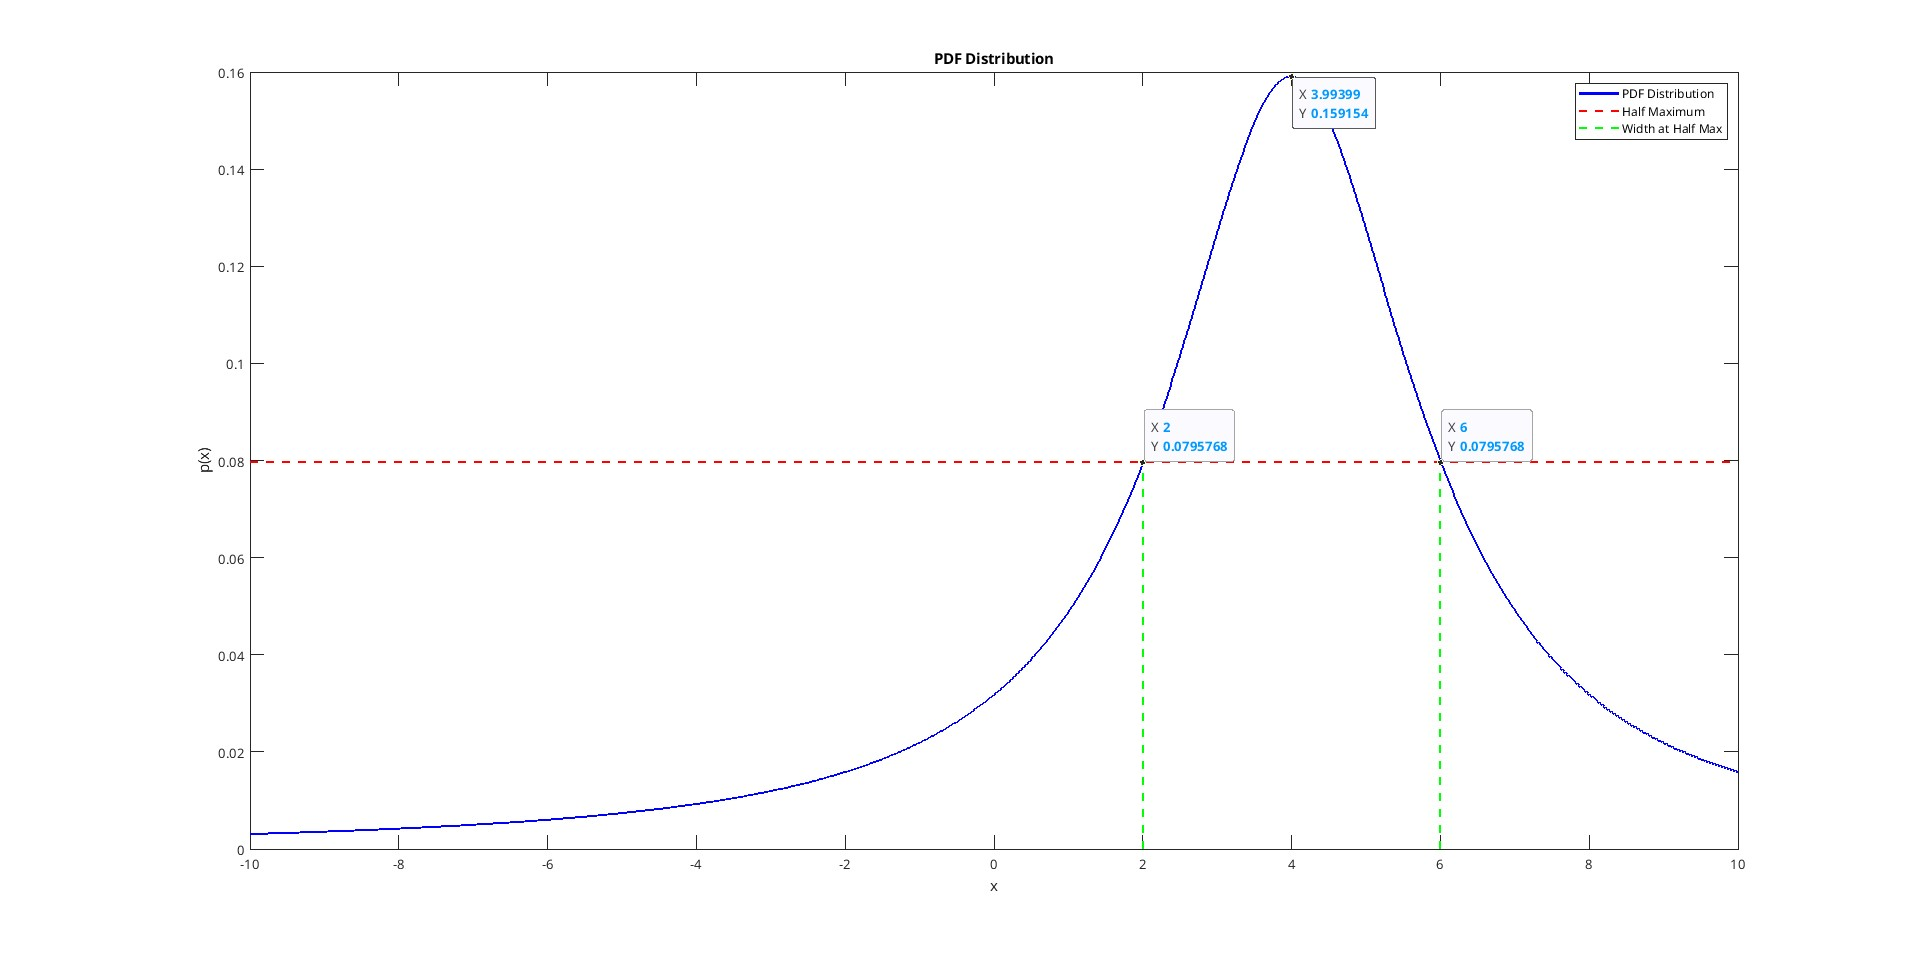
\includegraphics[scale=0.16]{q03pdfplot.jpg} \caption{Q3 Plot of the PDF $p(x_k | \alpha, \beta, B)$} \end{figure}

\section{QUESTION 4:}
Derive the expression for $p(\alpha | x_k, \beta, B)$.

\subsection*{Solution 4:} Using Bayes' Theorem, we derive the conditional distribution: \begin{equation} f_{\Lambda | X, \mathfrak{B},B} (\alpha | x_k, \beta) = \frac{f_{X | \Lambda, \mathfrak{B}, B}(x_k | \alpha, \beta) f_\Lambda(\alpha)}{f_X(x_k)} \end{equation} By applying similar techniques from Solution 2, the result is: \begin{equation} f_{\Lambda | X, \mathfrak{B}, B}(\alpha | x_k, \beta) = \frac{1}{\pi} \frac{\beta}{\beta^2 + (x_k - \alpha)^2} , \blacksquare \end{equation}

\section{QUESTION 5:}
Derive an expression for $p(\alpha | {x_k}^N _{k=1}, \beta, B)$. (State all assumptions.)

\subsection*{Solution 5:} Assumptions: \begin{itemize} \item The prior PDF is $f_{\Theta|\Lambda, \mathfrak{B},B}(\cdot) = \frac{1}{\pi}$. \item The measurements ${x_k}{k=1}^N$ are inputs to the random variable $X_k(\cdot)$. \item The measurements are independent and continuous. \end{itemize} The joint distribution of $p(\alpha | {x_k}^N{k=1}, \mathfrak{B}, B)$ is: \begin{equation} f_{\Lambda | X_k, \mathfrak{B},B} (\alpha | x_1,...,x_N, \beta) = \prod^N _{k=1} \frac{\beta}{\pi (\beta^2 + (x_k - \alpha)^2)} , \blacksquare \end{equation}

\section{QUESTION 6:}
Explain how one obtains the $x$-position of the robot from the result in (5).

\subsection*{Solution 6:} The $x$-position of the robot is determined by taking the product of the distributions of each $x_k$ measurement, as the measurements are independent. The $x$-position can also be obtained by locating the peak of the distribution or by using Maximum-A-Posteriori (MAP) estimation.

\section{QUESTION 7:}
Implement the Bayesian position inference scheme in MATLAB. Assume the robot is located inside a confined square region of size $10$m $\times$ $10$m. Demonstrate your Bayes estimator by inferring the robot’s $x$-position from the data ${ x_k }^{200}_{k=1}$ in \emph{BayesData.mat}, with the robot’s $y$-position at 4.5 m. Plot the Bayes posterior distribution for $N = 1, 2, 5,$ and $30$ measurements. What is your best $x$-position estimate?

\subsection*{Solution 7:} The MATLAB code implementing the Bayesian position inference scheme is provided in Appendix A, with the corresponding plots in Appendix B. For $N = 30$, the best estimate of $\alpha$ is approximately 5.86, as inferred from the posterior distribution. This is within the square region.

\section{QUESTION 8:}
The notation presented above deliberately does \emph{not} follow the conventions introduced by your Probability lecturer. Throughout your assignment, use the notation prescribed for use in the course.

\subsection*{Solution 8:} Yes, the following random variable notations are used: \begin{eqnarray} \Lambda (\cdot) = \alpha;: \mathfrak{B}(\cdot) = \beta ; : X(\cdot) = x_k; : \Theta ( \cdot) = \theta_k \ p(\theta_k | \alpha, \beta, B) = f_{\Theta | \Lambda, \beta, B}(, \cdot , | \alpha, \beta) \ p(\alpha | x_k, \beta, B) = f_{\Lambda | X, \mathfrak{B}, B}(, \cdot , | x_k, \beta) \ p(x_k |\alpha, \beta, B) = f_{X | \Lambda, \mathfrak{B}, B}(, \cdot , | \alpha, \beta) \end{eqnarray}

\section{QUESTION 9:}
Provide a professional report with clear and effective data representation. The report must not exceed 5 pages in length.

\subsection*{Solution 9:} This report follows the homework assignment format. References used include \cite{leon2017probability}, \cite{bishop2006pattern}.

\section{(Bonus) QUESTION 10:}
Infer both the $x$-position and the $y$-position of the robot. Estimate both $\alpha$ and $\beta$ for the PDF in Eq. (1).

\subsection*{Solution 10:} \emph{(Solution is to be provided.)}




\bibliographystyle{unsrt}
\bibliography{elen3007ref}

\newpage
\appendix

\makeatother
\section{Appendix A. - Matlab Inference Scheme Code}
\begin{lstlisting}[language=Matlab,
                   numbers=left,
                   basicstyle=\footnotesize,
                   stepnumber=1,
                   numbersep=10pt,
                   tabsize=2,
                   showspaces=false,
                   showstringspaces=false]
%%%%%%%%%Bayesian Position Inference Scheme%%%%%%%%%%%%
%numbat24.04%
%
% Main function to execute the Bayesian inference and plot results
function BayesianPositionInferenceScheme()
    load('BayesData.mat');
    % Given beta value and alpha range
    beta = 4.5;
    alpha_values = linspace(-50, 50, 1000);

    % Number of measurements to evaluate the posterior
    N_values = [1, 2, 5, 30];

    % Case 1: Points Inside the Box (0 <= x <= 10)
    x_inside_box = x(x >= 0 & x <= 10);
    plot_posterior(x_inside_box, N_values, alpha_values, beta, ...
        'Posterior for Points Inside the Box (0 <= x <= 10)');

    % Case 2: All Points (No Restrictions)
    x_all_points = x; 
    plot_posterior(x_all_points, N_values, alpha_values, beta, 
    'Posterior for All Points');
end

% Function to calculate the posterior for a given dataset and N points
function posterior_values = calculate_posterior(data, N, alpha_values, beta)
    posterior_values = zeros(size(alpha_values)); % Initialize posterior array
    for i = 1:length(alpha_values)
        alpha = alpha_values(i); % Current alpha value
        likelihood = 1; % Initialize likelihood as 1
        for k = 1:min(N, length(data))
            x_k_val = data(k);
            % Calculate the likelihood for each x_k_val
            likelihood = likelihood*(beta / (pi * (beta^2 + (x_k_val - alpha)^2)));
        end
        posterior_values(i) = likelihood; % Store posterior value
    end
    % Normalize the posterior to sum to 1
    posterior_values = posterior_values / sum(posterior_values);
end

% Function to plot the posterior for different N values
function plot_posterior(data, N_values, alpha_values, beta, title_text)
    figure; % Create new figure
    hold on;
    for N = N_values
        % Calculate posterior for the current N
        posterior_values = calculate_posterior(data, N, alpha_values, beta);
        % Plot the posterior distribution for this N
        plot(alpha_values, posterior_values, 'DisplayName', ['N = ', num2str(N)]);
    end
    xlabel('Alpha');
    ylabel('Posterior Probability');
    title(title_text);
    legend show;
    grid on;
    hold off;
end
\end{lstlisting}

\newpage
\section{Appendix B. - Matlab Scheme Plots}

\begin{figure}[h]
        \centering
        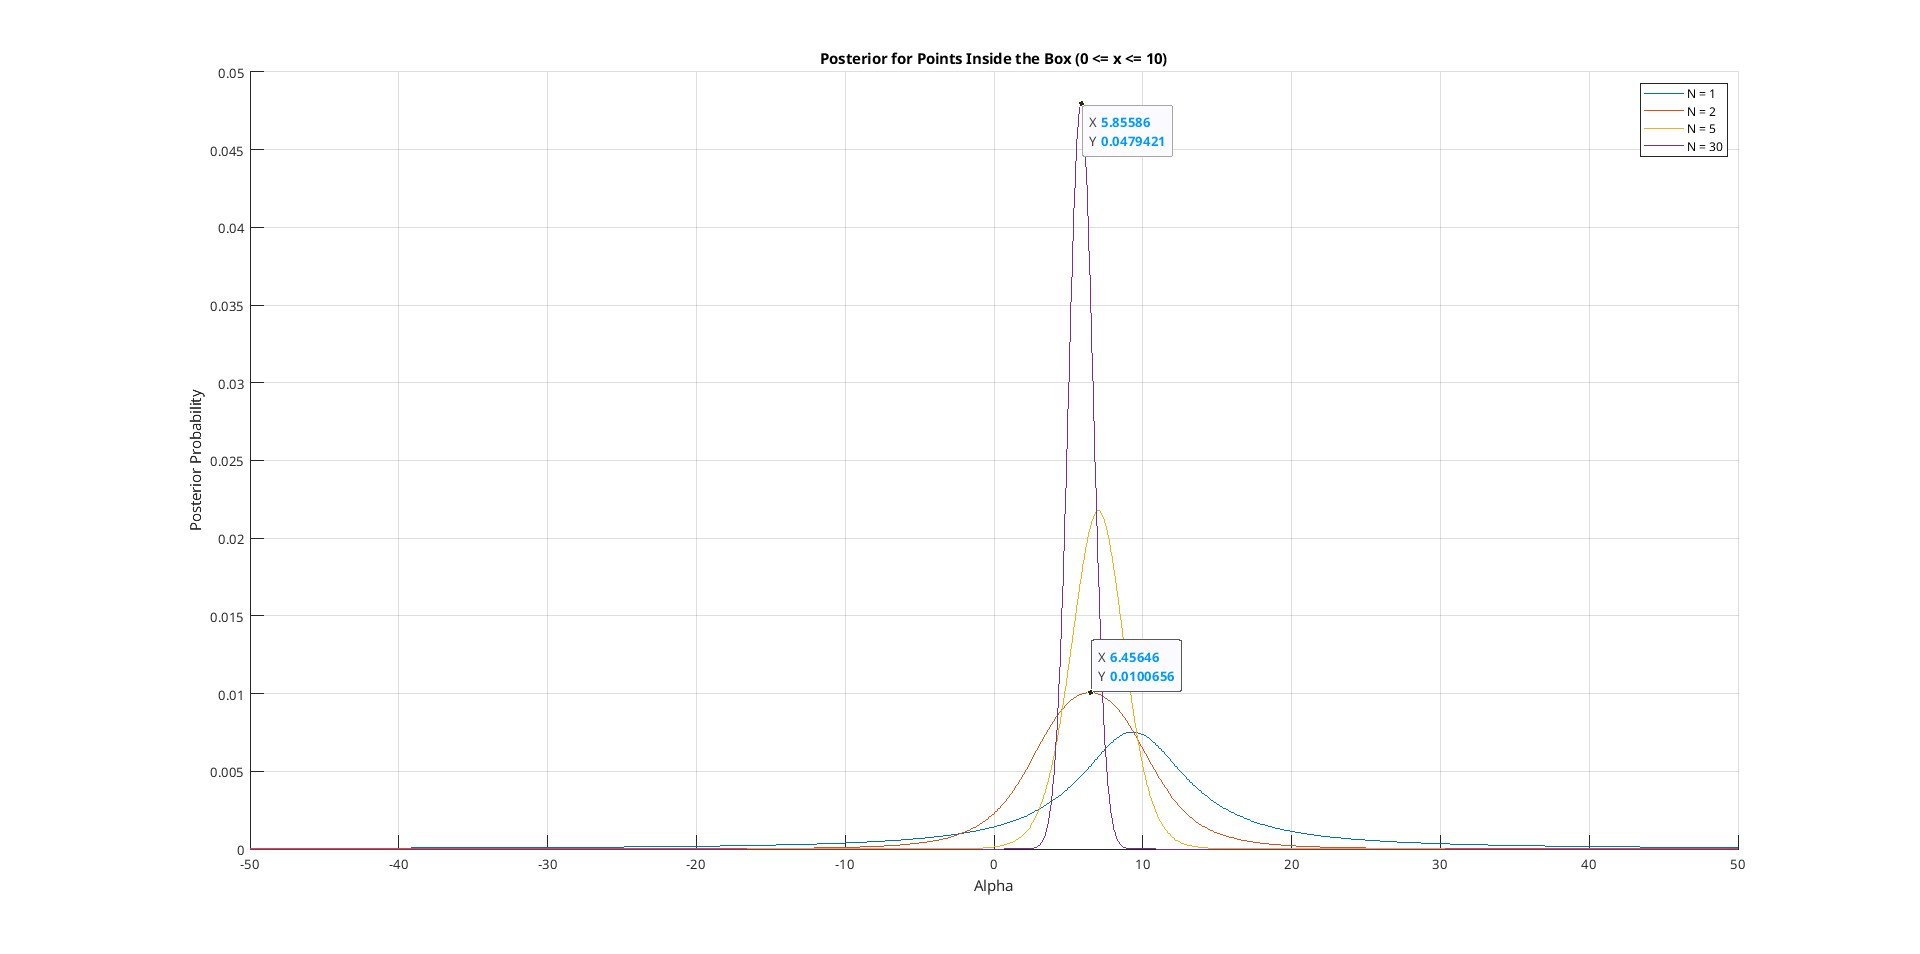
\includegraphics[scale=0.2]{q07pdfinbox.jpg} 
        \caption{Bayes' Inference Scheme Plot of the PDF for points inside the box}
\end{figure}	

\begin{figure}[h]
        \centering
        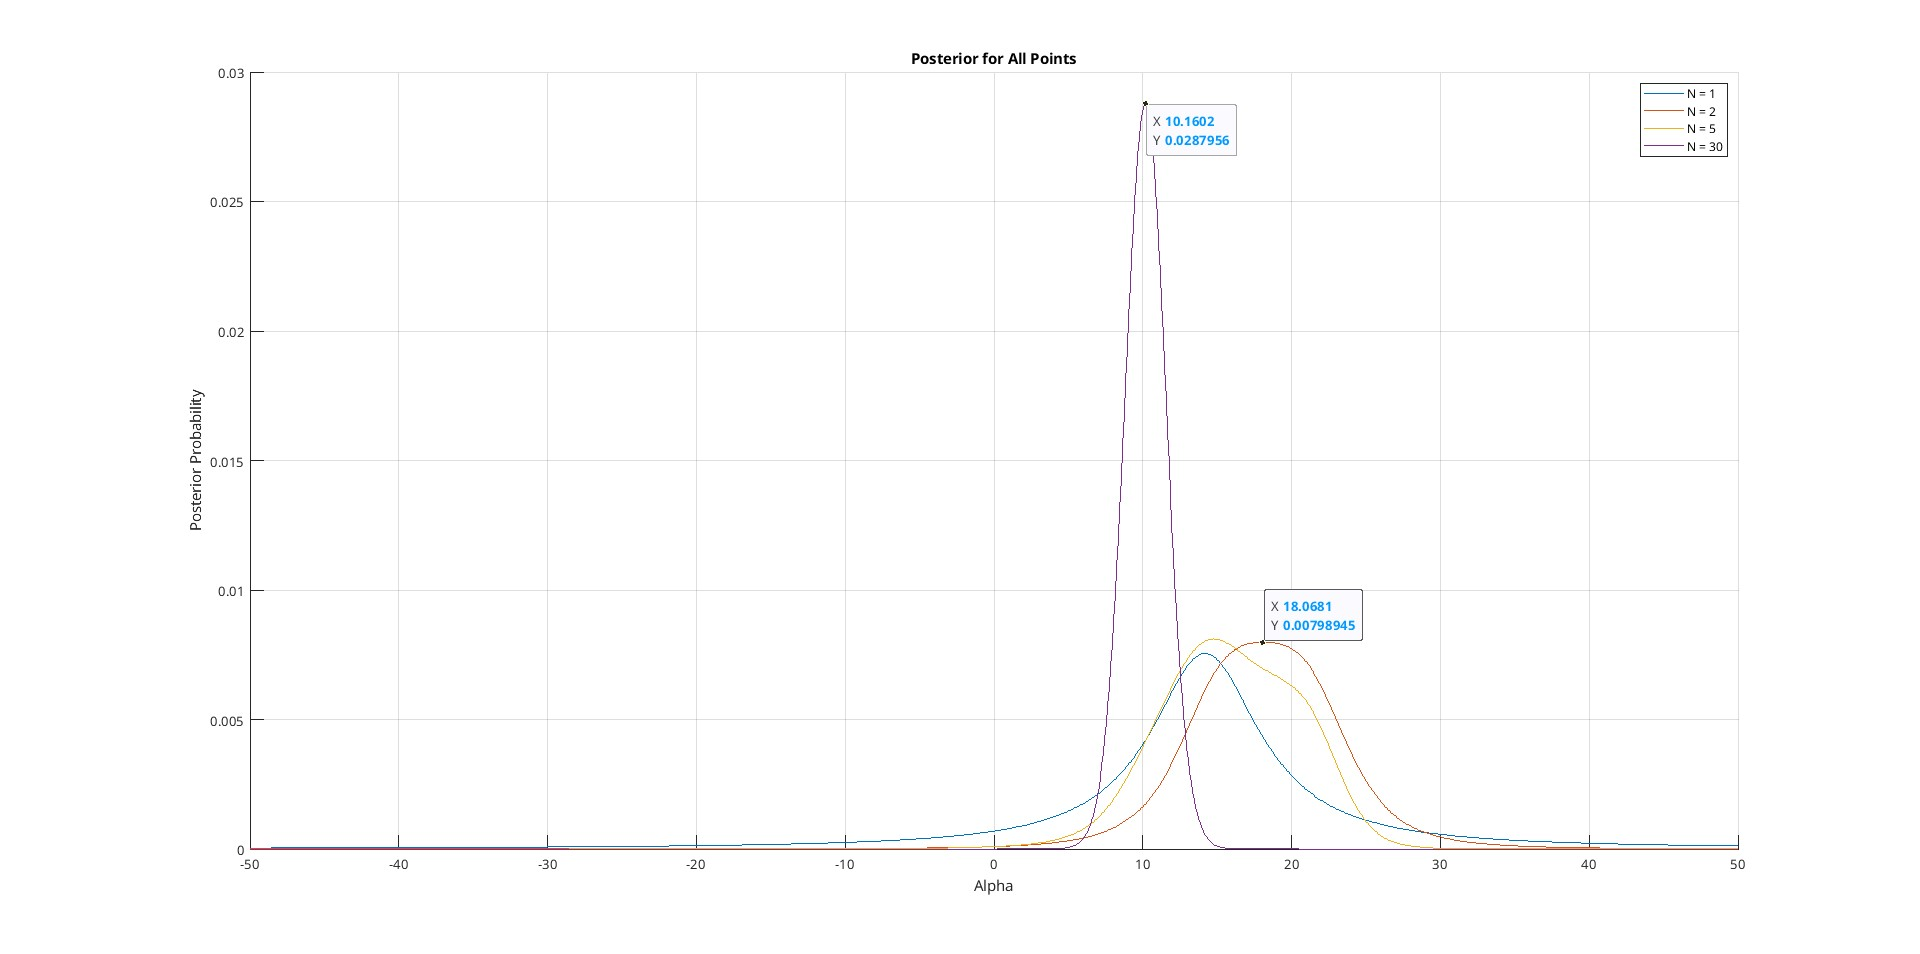
\includegraphics[scale=0.2]{q07pdfoutbox.jpg} 
        \caption{Bayes' Inference Scheme Plot of the PDF for all points}
\end{figure}	

\newpage
\section{Appendix C. - Maximul Likelyhood Estimation Scheme}
\begin{lstlisting}[language=Matlab,
                   numbers=left,
                   basicstyle=\small,
                   stepnumber=1,
                   numbersep=10pt,
                   tabsize=2,
                   showspaces=false,
                   showstringspaces=false]
%%%%%%%%%Estimating alpha using Maximum Likelyhood Solution%%%%%%%%%%%%
%numbat24.04%
%
% Load the data from BayesData.mat
load('BayesData.mat');

% Given y-position (beta)
beta = 4.5;

% Define the log-likelihood function so that product becomes a sum
log_likelihood = @(alpha) sum(log(beta ./ (pi * (beta^2 + (x - alpha).^2))));

% Find the alpha that maximizes the log-likelihood, 
% use fminsearch to minimize the negative log-likelihood, (equivalent to
% maximizing the likelihood)
alpha_mle = fminsearch(@(alpha) -log_likelihood(alpha), mean(x));

% Display the MLE result
disp(['Maximum Likelihood Estimate for alpha: ', num2str(alpha_mle)]);
%% alpha = 7.2287 %%
\end{lstlisting}

\end{document}